\begin{chapter}{Устойчивость двухкластерных вращательных режимов}
	\section{Устойчивость двух кластерных вращательных движений с постоянной расстройкой фаз}
	
	Запишем \ref{pre-pend} в виде системы:
	
	\begin{equation} \label{system}
		\begin{cases}
			\dot{x} = y, \\
			\dot{y} = \frac{1}{m} \left[ (1 - 2\beta)\sin{\alpha}(1 - \cos{x}) - \sin{x}\cos{\alpha} - y \right]
		\end{cases}
	\end{equation}
	
	Выполним линеаризацию системы \ref{system}:
	
	\begin{equation} \label{system-linear}
		\begin{pmatrix}
			\dot{\hat{x}} \\
			\dot{\hat{y}}
		\end{pmatrix}
		=
		\begin{pmatrix}
			0 & 1 \\
			\frac{1}{m}\left[ (1 - 2\beta)\sin{\alpha}\sin{x_p} - \cos{\alpha}\cos{x_p} \right] & -\frac{1}{m}
		\end{pmatrix}
		\begin{pmatrix}
			\hat{x} \\
			\hat{y}
		\end{pmatrix}
	\end{equation}
	Где $x_p$ - стационарные состояния уравнения \ref{pre-pend}. Запишем характеристический многочлен системы \ref{system-linear}:
	
	\begin{equation} \label{hp}
		\lambda^2 + \frac{1}{m}\lambda - \frac{1}{m}\left[ (1 - 2\beta)\sin{\alpha}\sin{x_p} - \cos{\alpha}\cos{x_p} \right] = 0
	\end{equation}
	
	Из \ref{hp} можно заметить, что устойчивость стационарного состояния $x_p$ определяется соотношением:
	
	\begin{equation} \label{hp-stability}
		\cos{\alpha}\cos{x_p} - (1 - 2\beta)\sin{\alpha}\sin{x_p} > 0
	\end{equation}
	
	Несложно заметить, что стационарные состояния в уравнении \ref{pre-pend} определяются:
	$$
	\sin{(x_p + \varphi)} = \frac{(1 - 2\beta) \sin{\alpha}}{\sqrt{\cos{\alpha}^2 + (1 - 2\beta)^2\sin{\alpha}^2}},
	$$
	Откуда:
	\begin{equation} \label{x1}
		x_{p_1} = \begin{cases}
			0, \alpha \in [-\pi/2, \pi/2) \\
			2\arcsin{\frac{(1 - 2\beta) \sin{\alpha}}{\sqrt{\cos{\alpha}^2 + (1 - 2\beta)^2\sin{\alpha}^2}}} - \pi , \alpha \in [\pi/2, 3\pi/2)
		\end{cases}
	\end{equation}
	
	\begin{equation} \label{x2}
	x_{p_2} = \begin{cases}
		\pi - 2\arcsin{\frac{(1 - 2\beta) \sin{\alpha}}{\sqrt{\cos{\alpha}^2 + (1 - 2\beta)^2\sin{\alpha}^2}}}, \alpha \in [-\pi/2, \pi/2) \\
		0, \alpha \in [\pi/2, 3\pi/2)
		\end{cases}
	\end{equation}
	
	Подставляя \ref{x1}, \ref{x2} в \ref{hp-stability}
	получаем, что $x_{p_1}$ - устойчива, $x_{p_2}$ - неустойчива.

	\begin{figure}[h!]\center
		\begin{tabular}{cc}
		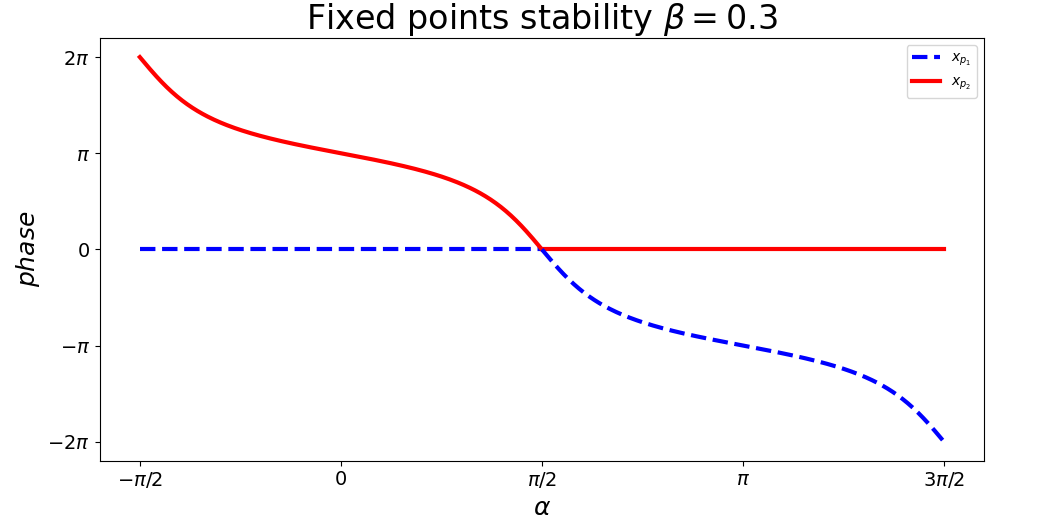
\includegraphics[width=0.54\columnwidth]{pictures/fixed-points.png}
		&
		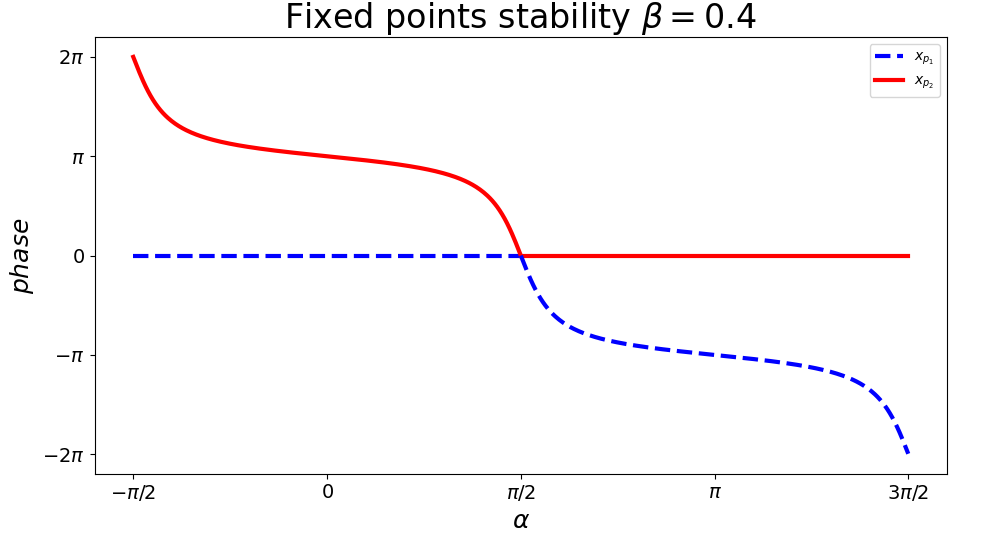
\includegraphics[width=0.5\columnwidth]{pictures/fixed-points-2.png} 
		\end{tabular}
		\caption{\textbf{Устойчивость стационарных состояний.}
		Синяя пунктирная линия - устойчивое состояние $x_{p_1}$,
		Красная сплошная линия - неустойчивое состояние $x_{p_2}$.
		$\beta = 0.3$, $\beta = 0.4$}
	\end{figure}

	\begin{figure}[h!]
		\begin{center}
			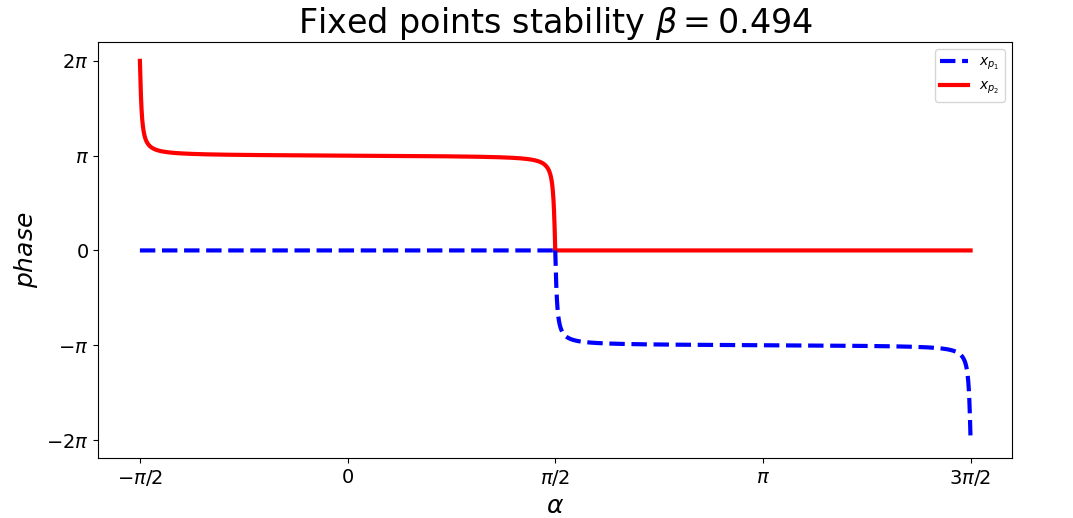
\includegraphics[width=1\columnwidth]{pictures/fixed-points-3.png}
		\end{center}
		\caption{\textbf{Устойчивость стационарных состояний.}
		Синяя пунктирная линия - устойчивое состояние $x_{p_1}$,
		Красная сплошная линия - неустойчивое состояние $x_{p_2}$.
		$\beta = 0.494$}
	\end{figure}

	Заметим, что при $\beta$ стремящейся к 0.5 стационарные состояния с расстройкой фаз неравной нулю стремятся
	к $\pi k$, $k \in \mathbb{Z}$.
	Стоит отметить, что в полной системе \ref{main-sistem} стационарное двух кластерное состояние $x_{p_1}$
	может терять свою устойчивость. Данный эффект будет показан ниже.
	
	\section{Устойчивость двух кластерных вращательных движений с периодической расстройкой фаз}

	Выполним линеаризацию относительно произвольного вращательного движения $\psi_i$ с помощью замены
	$\varphi_i = \psi_i + \delta_i$:
	\begin{equation}
		m\ddot{\delta}_i + \dot{\delta}_i = \frac{1}{N} \sum_{j = 1}^N \cos{(\psi_j - \psi_i - \alpha)} \cdot (\delta_j - \delta_i), \ i = \overline{1, N}
	\end{equation}
	Для случая двух кластерного режима \ref{two-cluster} это запишется в виде:
	
	\begin{equation}
		\begin{cases}
			m\ddot{\delta}_i + \dot{\delta}_i = \frac{1}{N} \left( \cos{\alpha} \sum_{j = 1}^K (\delta_j - \delta_i) + \cos{(X + \alpha)} \sum_{j = K + 1}^N (\delta_j - \delta_i) \right), \ i = \overline{1,K}, \\
			m\ddot{\delta}_i + \dot{\delta}_i = \frac{1}{N} \left( \cos{(X - \alpha)} \sum_{j = 1}^K (\delta_j - \delta_i) +  \cos{\alpha} \sum_{j = K + 1}^N (\delta_j - \delta_i)  \right), \ i = \overline{K + 1,N},
		\end{cases}		
	\end{equation}
	
	Выполняя замену:
	\begin{align*}
		\eta_1 = \frac{1}{K} \sum_{i = 1}^K \delta_i - \frac{1}{N - K} \sum_{i = K + 1}^N \delta_i, \\
		\eta_2 = \frac{1}{K} \sum_{i = 1}^K \delta_i + \frac{1}{N - K} \sum_{i = K + 1}^N \delta_i, \\
		\xi_n = \delta_{n+1} - \delta_n, \ 1 \leq  n \leq K - 1, \\
		\zeta_n = \delta_{n+1} - \delta_n, \ K + 1 \leq n \leq N - 1.
	\end{align*}
		
	Мы получаем:
	
	\begin{equation} \label{split-linear-pert-sys-n12}
		\begin{cases}
			m\ddot{\eta}_1 + \dot{\eta}_1 + \left( \beta \cos{(X - \alpha)} + (1 - \beta) \cos{(X + \alpha)} \right) \eta_1 = 0, \\
			m\ddot{\eta}_2 + \dot{\eta}_2 + \left( (1 - \beta) \cos{(X + \alpha)} - \beta \cos{(X - \alpha)} \right) \eta_1 = 0,
		\end{cases}
	\end{equation}
	
	
	\begin{equation} \label{split-linear-pert-sys-ksi-eta}
		\begin{cases}
			m\ddot{\xi}_n + \dot{\xi}_n + \left( (1 - \beta) \cos{(X + \alpha)} + \beta \cos{\alpha} \right) \xi_n = 0, \\
			m\ddot{\zeta}_n + \dot{\zeta}_n + \left( (1 - \beta) \cos{\alpha} + \beta \cos{(X - \alpha)} \right) \zeta_n = 0.
		\end{cases}
	\end{equation}
	
	Так как $X$ периодична, мы можем применить теорию Флоке
	и найти мультипликаторы, определяющие асимптотическое поведение решений системы.
	
	Проанализируем систему \ref{split-linear-pert-sys-n12} (переменные $\eta_1$, $\eta_2$).
	Из \ref{pre-pend} следует, что одним из
	решений первого уравнения является $\dot{X}$.
	Так как $X$ периодична, то один из мультипликаторов равен 1.
	Согласно формуле Лиувилля-Остроградского, второй мультипликатор первого уравнения равен $\exp{(-\frac{T_x}{m})}$.
	Кроме того, полная система имеет решение $\eta_1 = 0$, $\eta_2 = const$,
	откуда следует, что еще один мультипликатор равен единице.
	Вновь применяя формулу Лиувилля-Остроградского, но
	уже ко всей системе, находим четвертый мультипликатор,
	равный $\exp{(-\frac{T_x}{m})}$. 
	Итак, режим всегда внутренне устойчив.
	
	
	Проанализируем систему \ref{split-linear-pert-sys-ksi-eta} (переменные $\xi$, $\zeta$).
	Переменная $\xi$ соответствует малому кластеру, переменная $\zeta$ соответствует большому кластеру. 
	Они не связанны между собой.
	Благодаря такому разделению переменных, мы можем проследить как меняется устойчивость
	двух кластерного режима с периодической расстройкой фаз для каждого кластера. В зависимости от $X$ устойчивость
	может пропасть или появится только у одного или сразу у двух кластеров, благодаря чему мы можем
	понять каким образом двух кластерный режим будет разрушаться в случае потери устойчивости.
	
	С помощью уравнений \ref{split-linear-pert-sys-ksi-eta} определим устойчивость стационарного
	двух кластерного вращательного режима, соответствующего состоянию $x_{p_1}$.
	Уравнения запишутся в виде:
	
	\begin{equation}
		x_{p_1} = 0, \ \alpha \in [-\pi/ 2, \pi/2]: 
		\begin{cases}
			m\ddot{\xi}_n + \dot{\xi}_n + \cos{\alpha}\xi_n = 0, \\
			m\ddot{\zeta}_n + \dot{\zeta}_n + \cos{\alpha}\zeta_n = 0.
		\end{cases}
	\end{equation}
	
	\begin{equation}
		\begin{split}
			x_{p_1} = 2\arcsin{\frac{(1 - 2\beta) \sin{\alpha}}{\sqrt{\cos{\alpha}^2 + (1 - 2\beta)^2\sin{\alpha}^2}}} - \pi , \alpha \in [\pi/2, 3\pi/2): \\ 
			:\begin{cases}
				m\ddot{\xi}_n + \dot{\xi}_n + A(\alpha, \beta) \xi_n = 0, \\
				m\ddot{\zeta}_n + \dot{\zeta}_n -A(\alpha, \beta) \zeta_n = 0.
			\end{cases}
		\end{split}
	\end{equation}
	Где $A$ - некоторый коэффициент. Заметим, что при $\alpha \in [-\pi/ 2, \pi/2)$, $x_{p_1}$ - устойчива в исходной системе,
	при $\alpha \in [\pi/2, 3\pi/2)$, $x_{p_1}$ - неустойчива в исходной системе.

	Получается, что в исходной системе двухкластерный вращательный режим с постоянной расстройкой фаз всегда является неустойчивым.
	Таким образом дальнейший анализ устойчивости мы будем проводить только для двухкластерных вращательных движений с периодической
	расстройкой фаз.


	В результате численного моделирования были получены карты устойчивости двух кластерных вращательных
	режимов с периодической расстройкой фаз в области параметров $\alpha$, $m$.

	\begin{figure}[h!]\center
		\begin{tabular}{cc}
		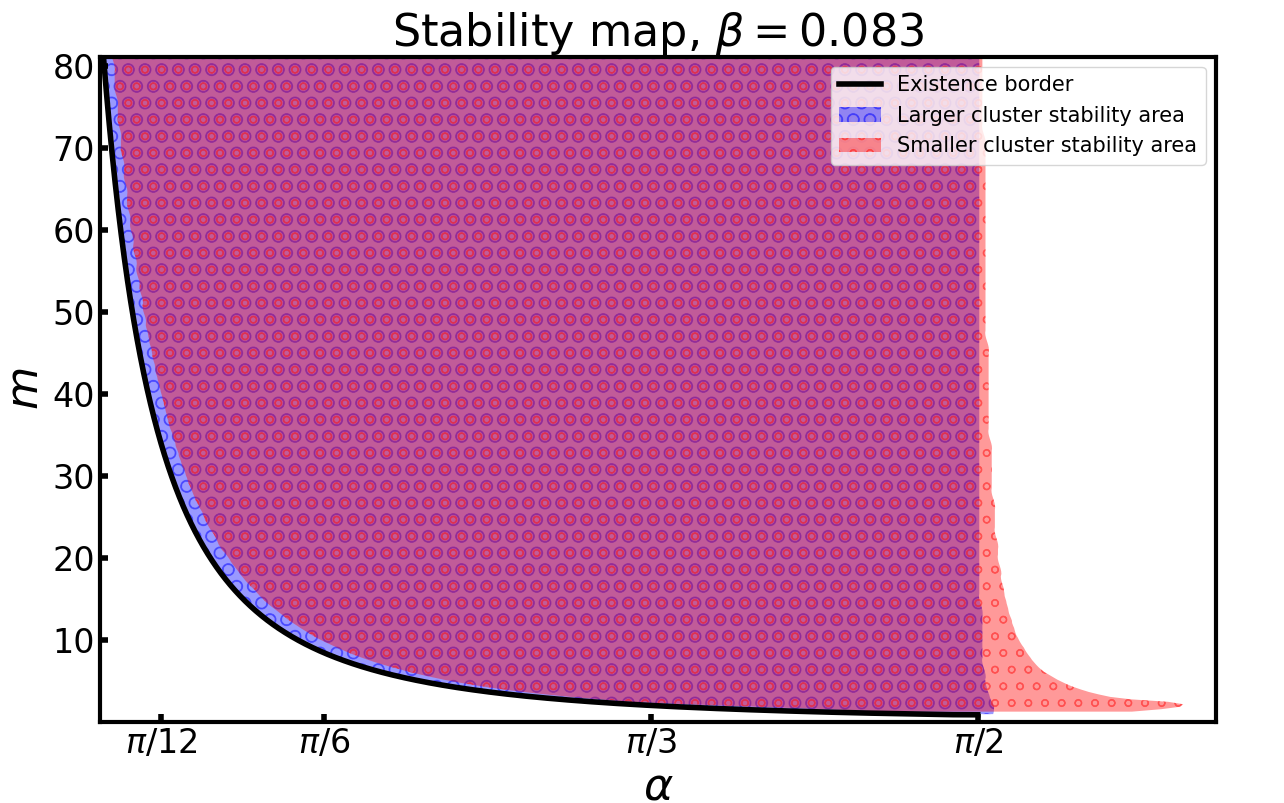
\includegraphics[width=0.5\columnwidth]{pictures/map-0-083.png}
		&
		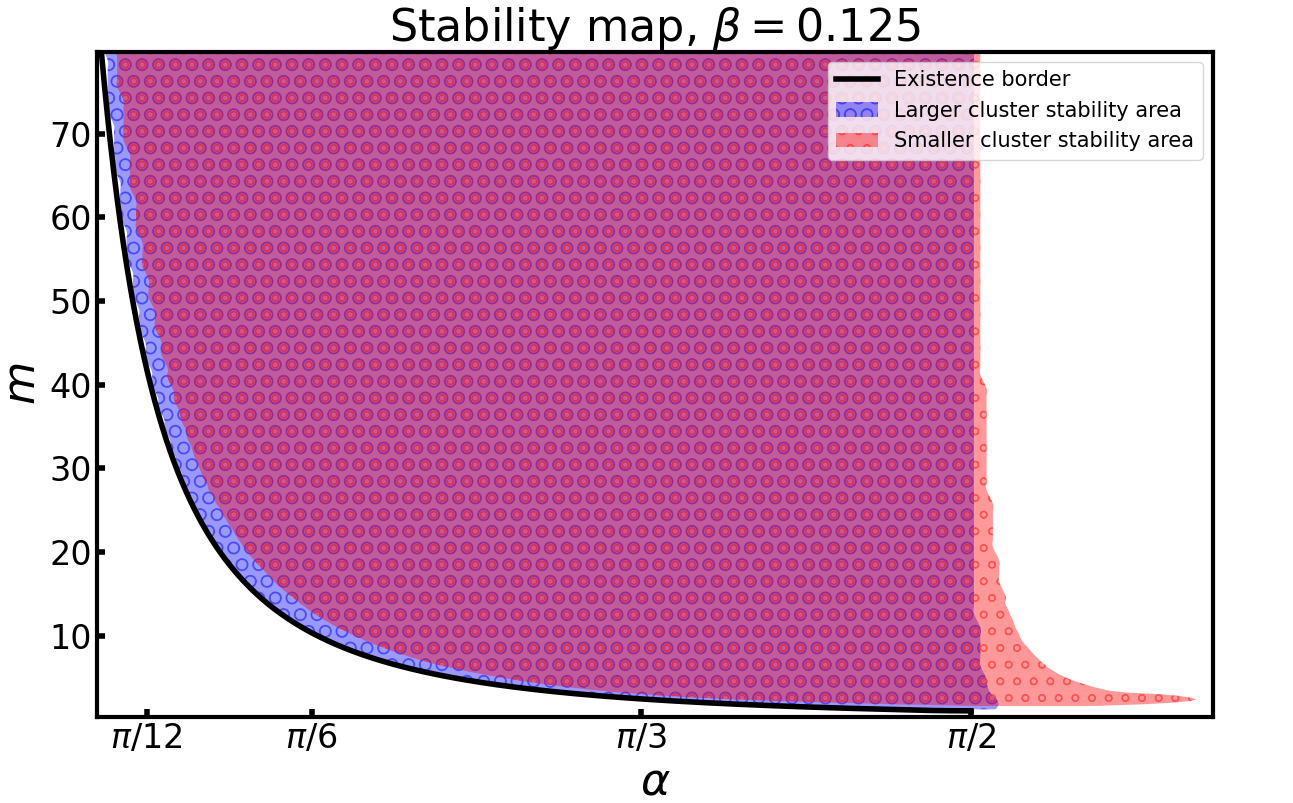
\includegraphics[width=0.5\columnwidth]{pictures/map-0-0125.png}
		\end{tabular}
		\caption{\textbf{Карта устойчивости двух кластерных вращательных состояний с периодической расстройкой фаз.}
		Область с малыми маркерами соответствует устойчивости малого кластера.
		Область с большими маркерами соответствует устойчивости большого кластера.
		На пересечении этих областей двух кластерный вращательный режим с периодической расстройкой фаз является устойчивым}
	\end{figure}

	
	\begin{figure}[h!]\center
		\begin{tabular}{cc}
		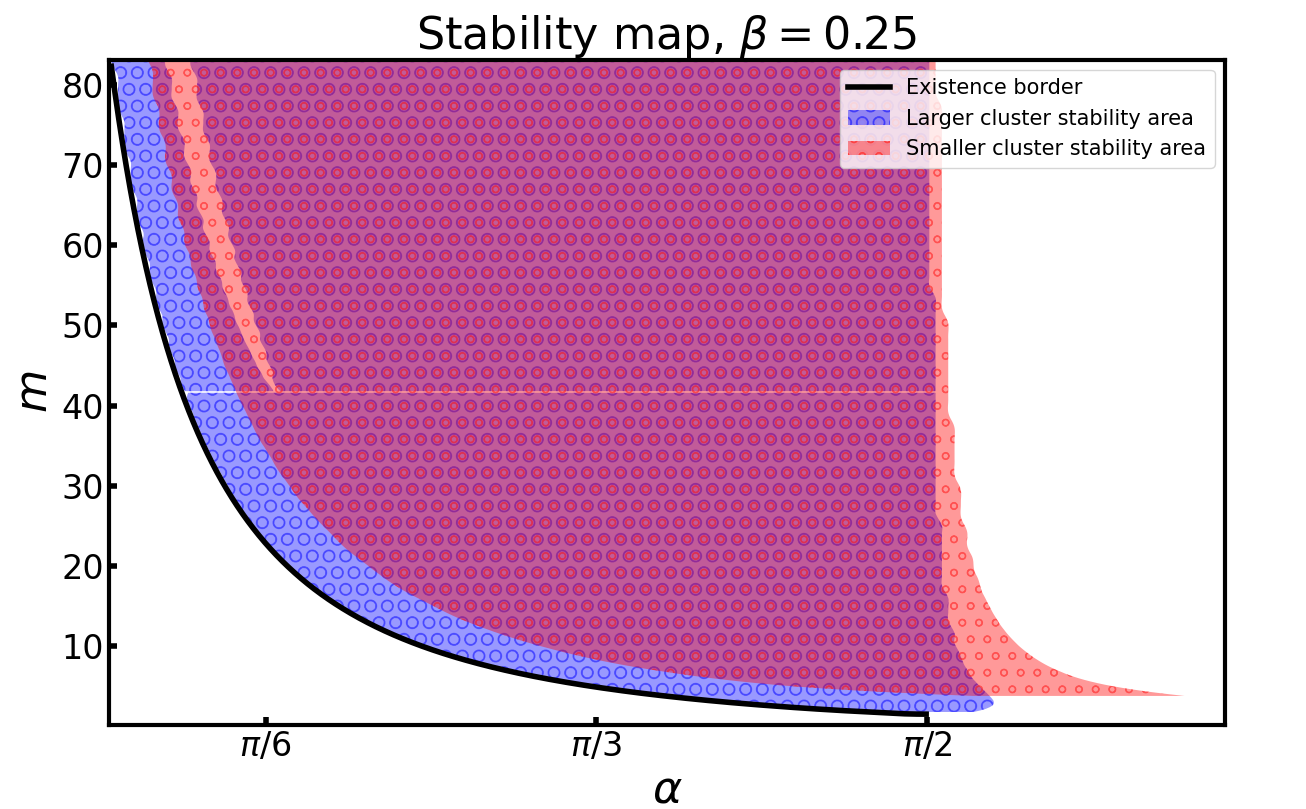
\includegraphics[width=0.5\columnwidth]{pictures/map-0-25.png}
		&
		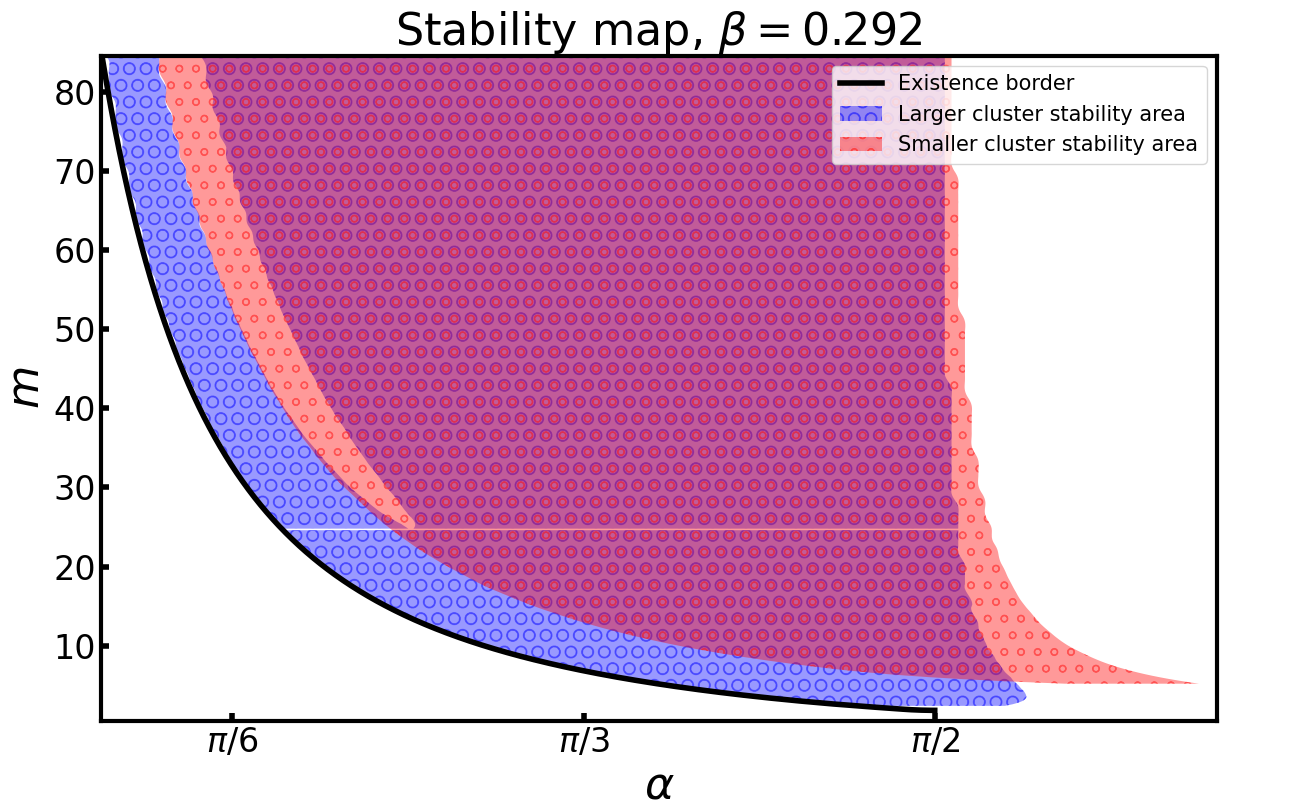
\includegraphics[width=0.5\columnwidth]{pictures/map-0-292.png}
		\end{tabular}
		\caption{\textbf{Карта устойчивости двух кластерных вращательных состояний с периодической расстройкой фаз.}
		Область с малыми маркерами соответствует устойчивости малого кластера.
		Область с большими маркерами соответствует устойчивости большого кластера.
		На пересечении этих областей двух кластерный вращательный режим с периодической расстройкой фаз является устойчивым}
		\label{map-025}
	\end{figure}

	\begin{figure}[h!]\center
		\begin{tabular}{cc}
		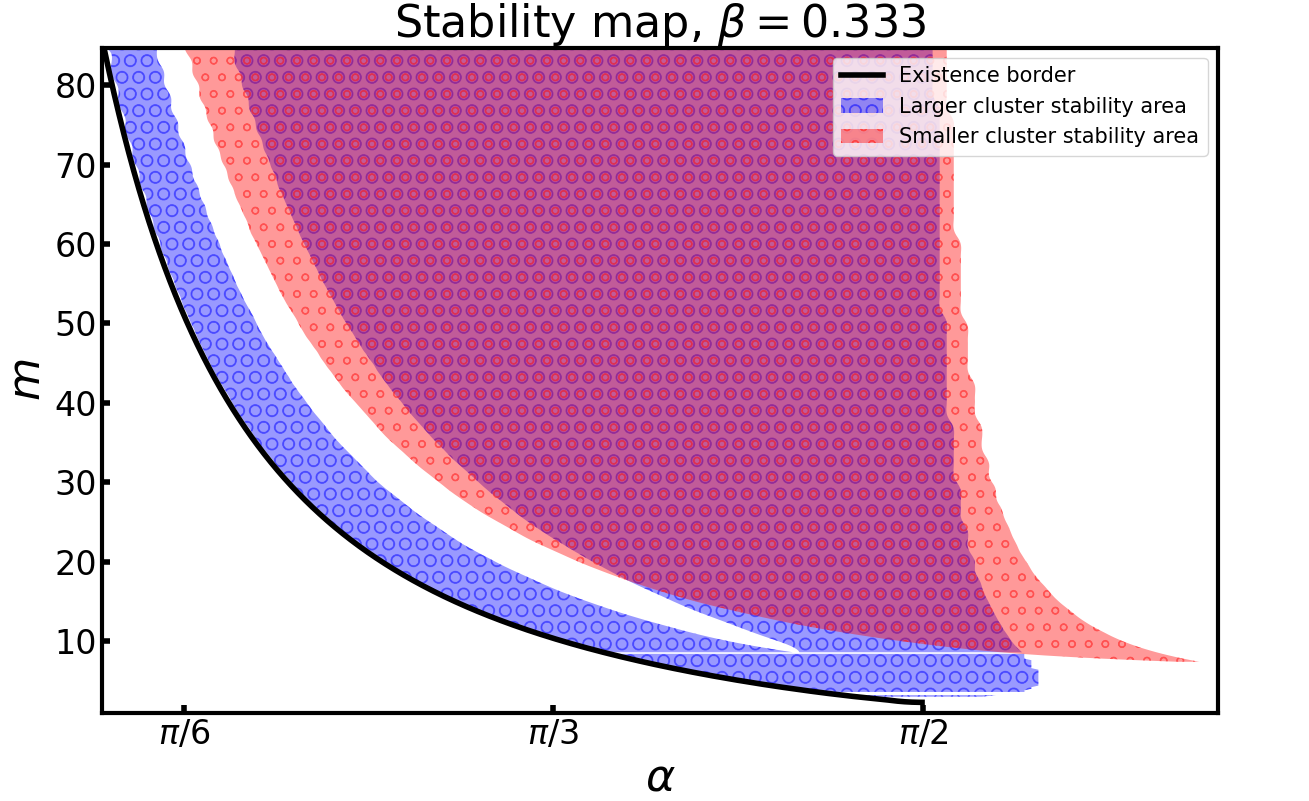
\includegraphics[width=0.5\columnwidth]{pictures/map-0-33.png}
		&
		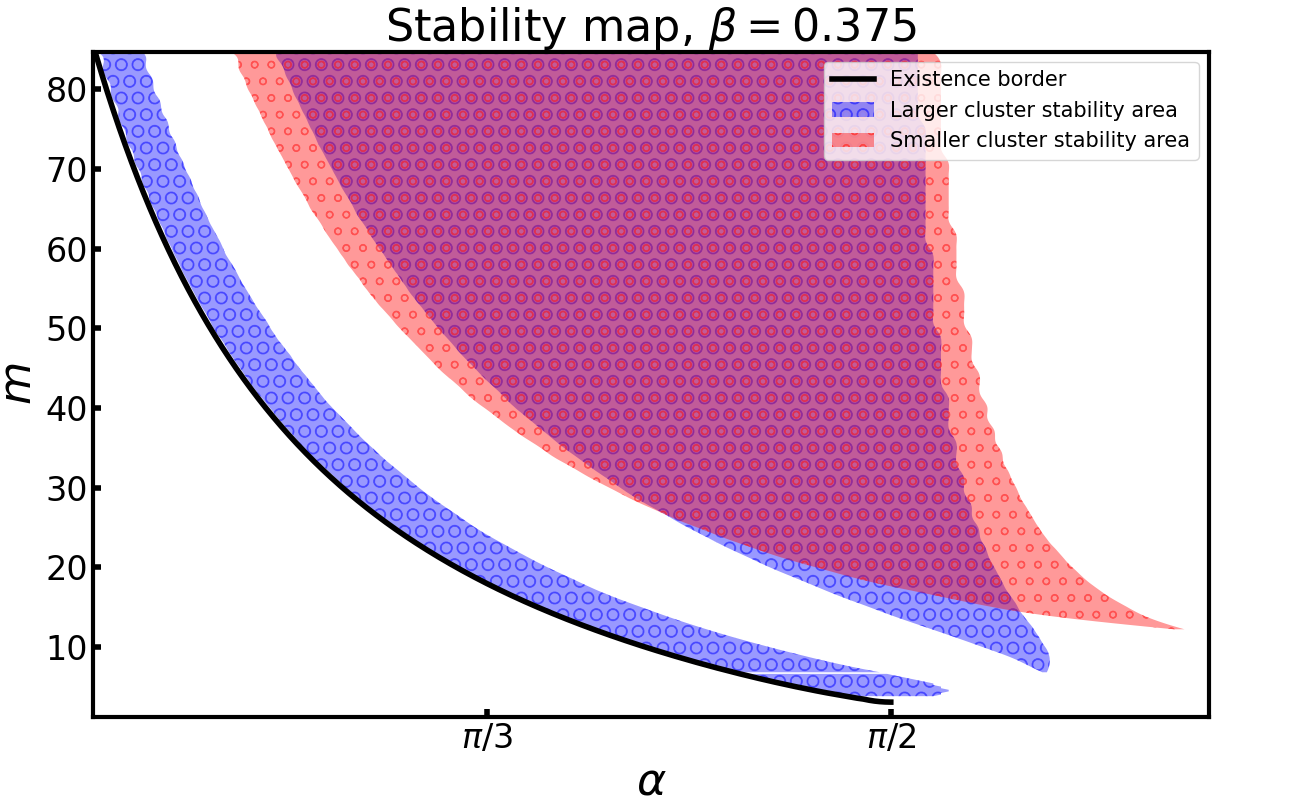
\includegraphics[width=0.5\columnwidth]{pictures/map-0-375.png}
		\end{tabular}
		\caption{\textbf{Карта устойчивости двух кластерных вращательных состояний с периодической расстройкой фаз.}
		Область с малыми маркерами соответствует устойчивости малого кластера.
		Область с большими маркерами соответствует устойчивости большого кластера.
		На пересечении этих областей двух кластерный вращательный режим с периодической расстройкой фаз является устойчивым}
	\end{figure}

	


	\begin{figure}[h!]\center
		\begin{tabular}{cc}
		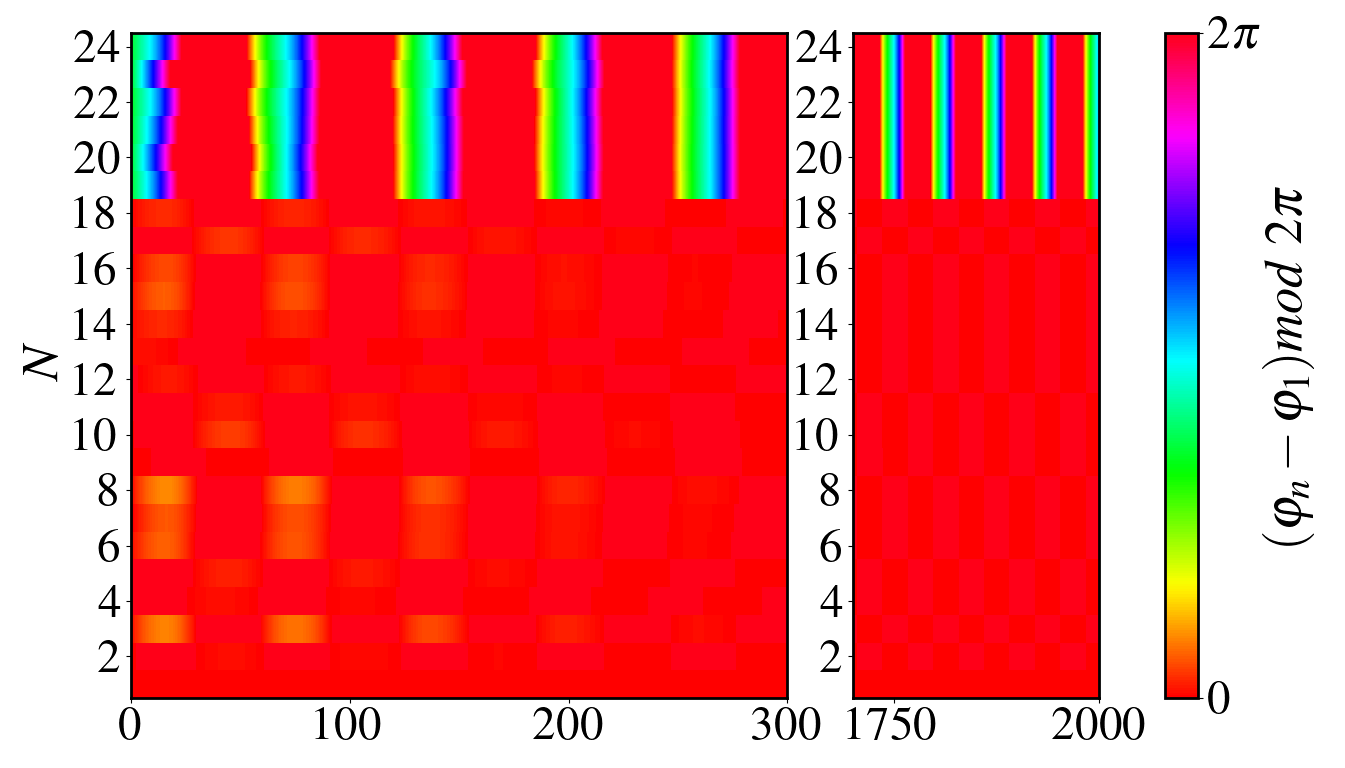
\includegraphics[width=0.5\columnwidth]{pictures/Figure_M_50_A_0.4586_O_1.png}
		&
		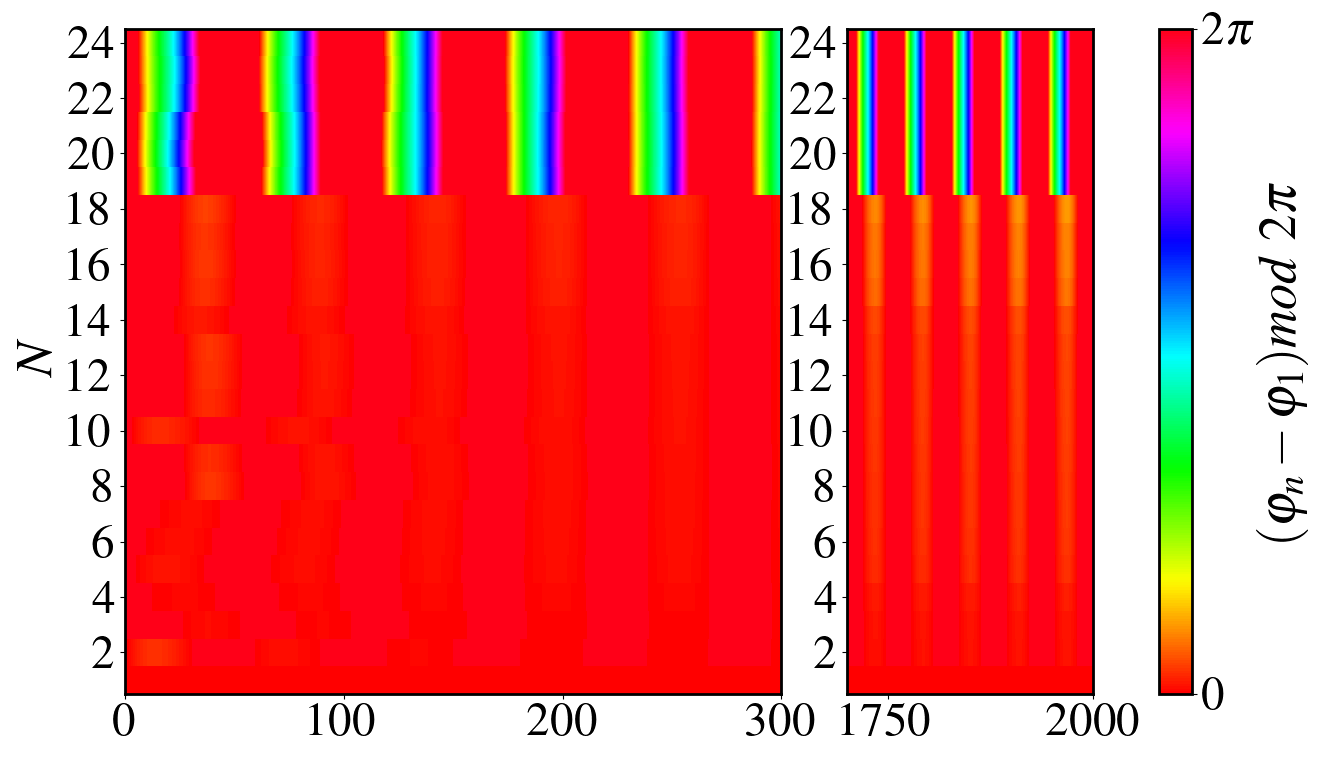
\includegraphics[width=0.5\columnwidth]{pictures/Figure_M_50_A_0.4946_O_1.png}
		\end{tabular}
		\caption{\textbf{Карта устойчивости двух кластерных вращательных состояний с периодической расстройкой фаз.}
		Область с малыми маркерами соответствует устойчивости малого кластера.
		Область с большими маркерами соответствует устойчивости большого кластера.
		На пересечении этих областей двух кластерный вращательный режим с периодической расстройкой фаз является устойчивым}
	\end{figure}


	% \begin{figure}[h!]
	% 	\begin{center}
	% 		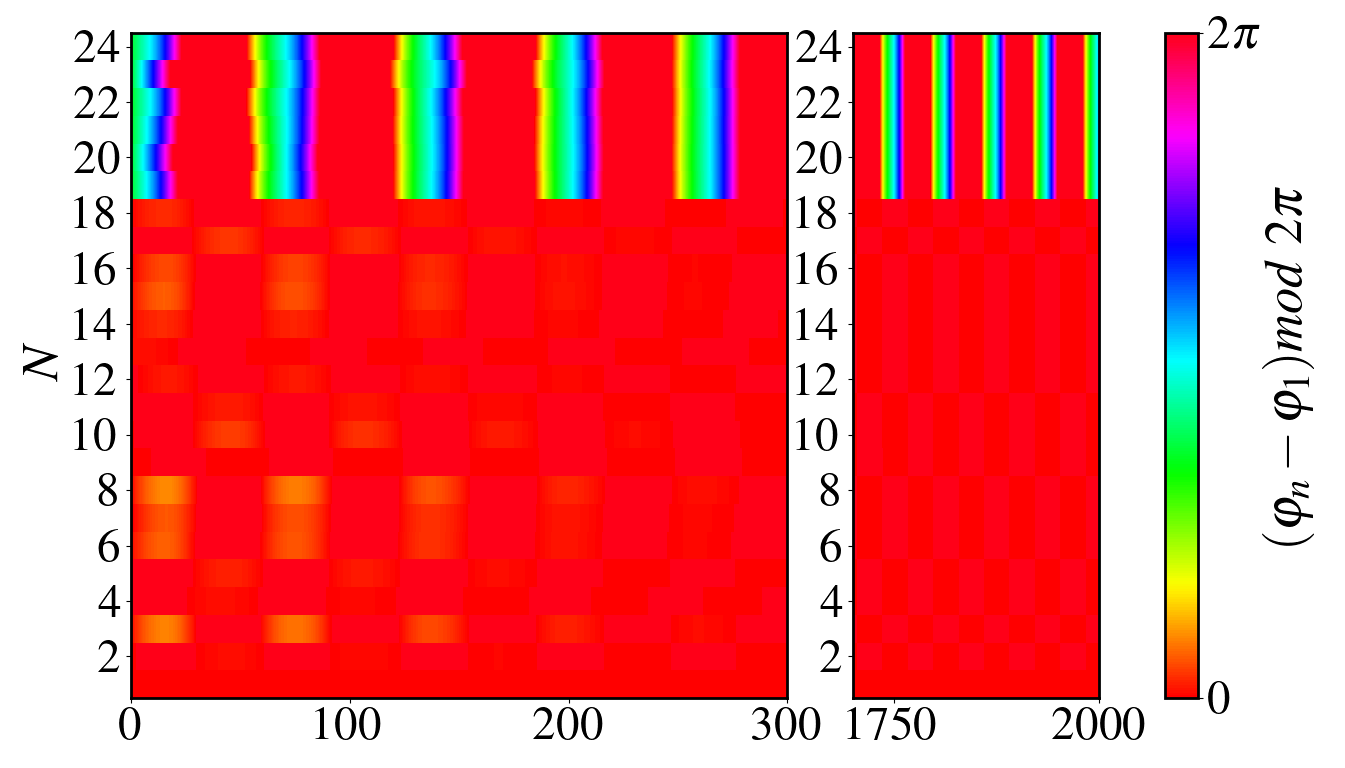
\includegraphics[width=1\columnwidth]{pictures/Figure_M_50_A_0.4586_O_1.png}
	% 	\end{center}
	% 	\caption{\textbf{Пространственно временная диаграмма.}
	% 	Пространственно временные диаграммы изображены для каждого элемента, относительно первого элемента.
	% 	Цвет характеризует фазу элемента. Параметры: $N=24$, $m = 50$, $\omega = 1$, $\alpha = 0.4586$ (см. рис. \ref{map-025})}
	% \end{figure}
	
	% \begin{figure}[h!]
	% 	\begin{center}
	% 		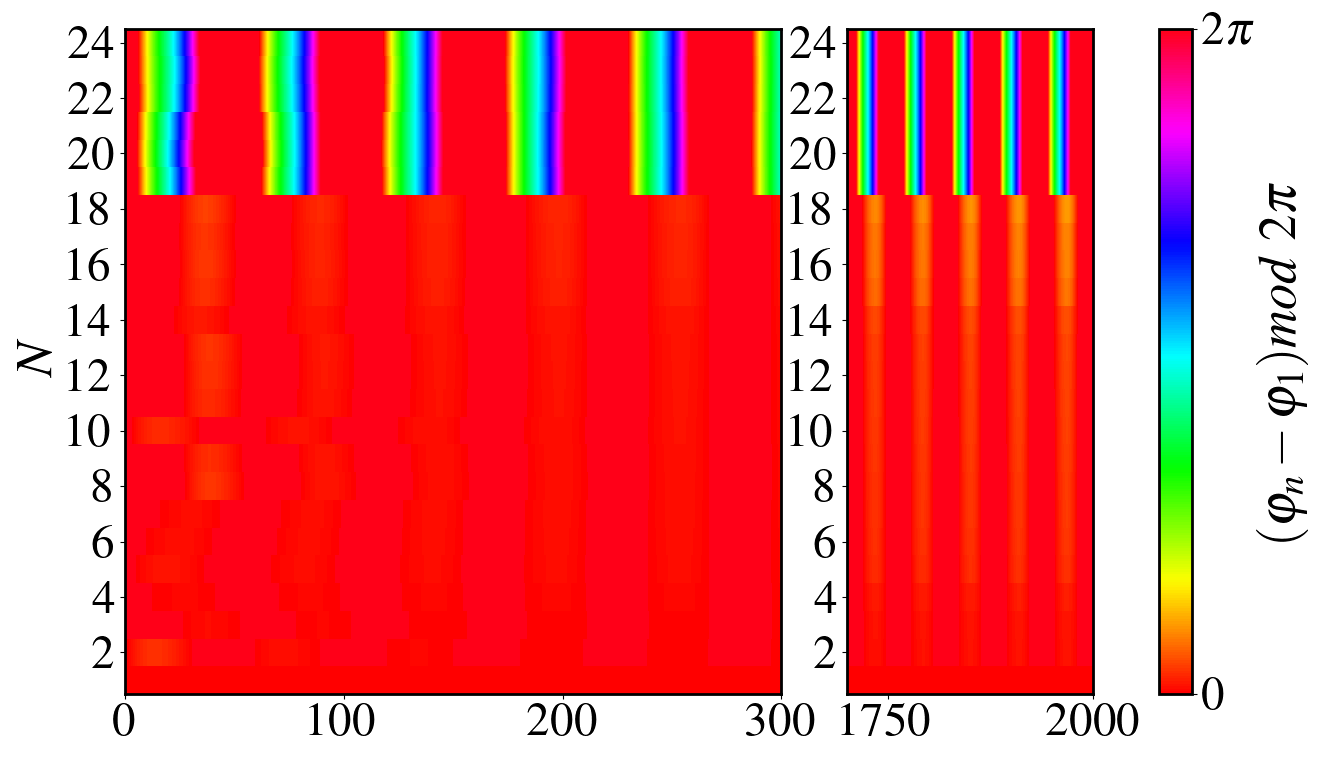
\includegraphics[width=1\columnwidth]{pictures/Figure_M_50_A_0.4946_O_1.png}
	% 	\end{center}
	% 	\caption{\textbf{Пространственно временная диаграмма.}
	% 	Пространственно временные диаграммы изображены для каждого элемента, относительно первого элемента.
	% 	Цвет характеризует фазу элемента. Параметры: $N=24$, $m = 50$, $\omega = 1$, $\alpha = 0.4946$ (см. рис. \ref{map-025})}
	% \end{figure}
	
	\begin{figure}[h!]
		\begin{center}
			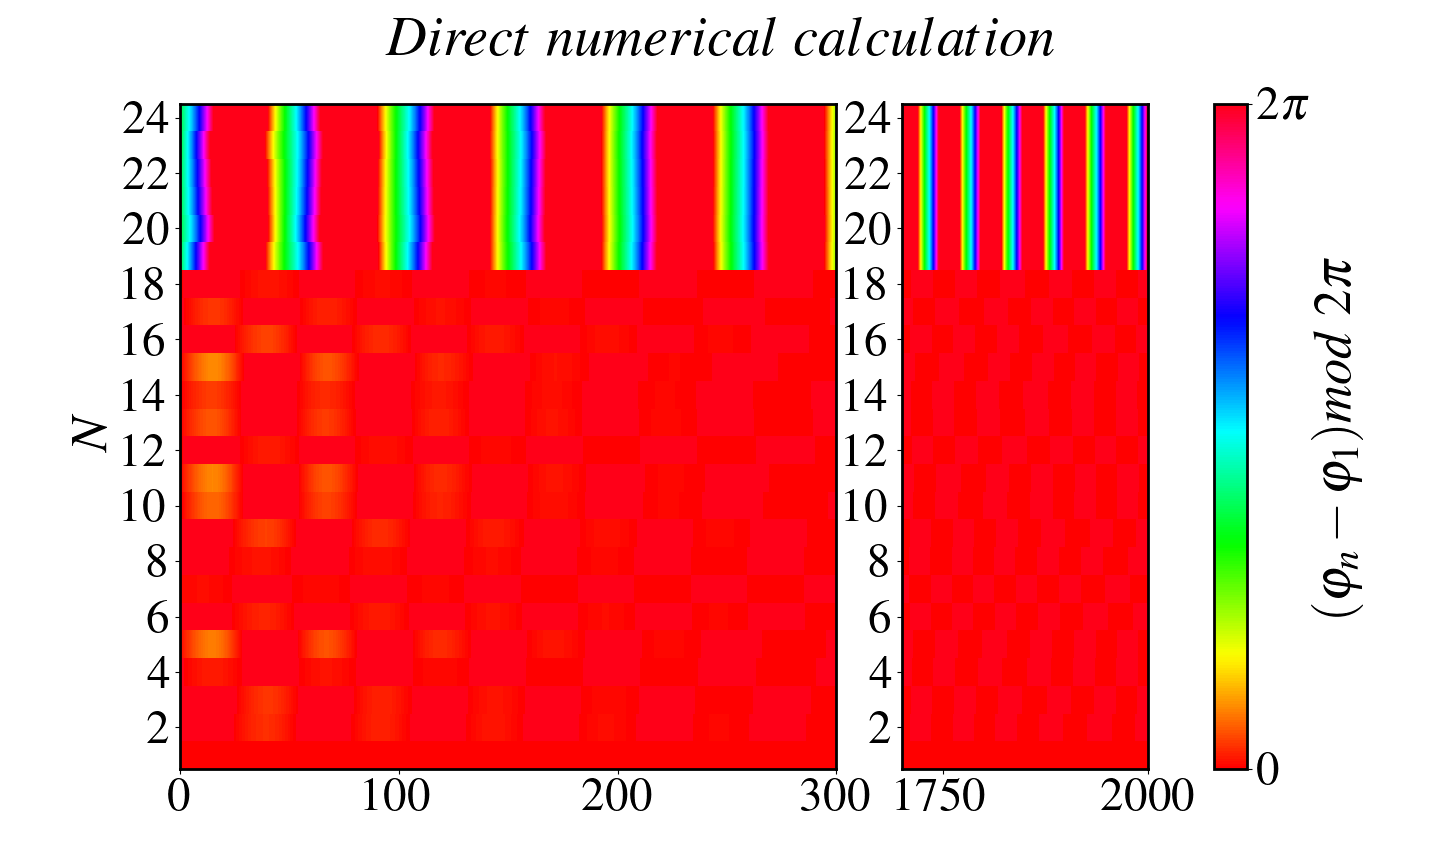
\includegraphics[width=1\columnwidth]{pictures/Figure_M_50_A_0.54_O_1.png}
		\end{center}
		\caption{\textbf{Пространственно временная диаграмма.}
		Пространственно временные диаграммы изображены для каждого элемента, относительно первого элемента.
		Цвет характеризует фазу элемента. Параметры: $N=24$, $m = 50$, $\omega = 1$, $\alpha = 0.54$ (см. рис. \ref{map-025})}
	\end{figure}

	\begin{figure}[h!]
		\begin{center}
			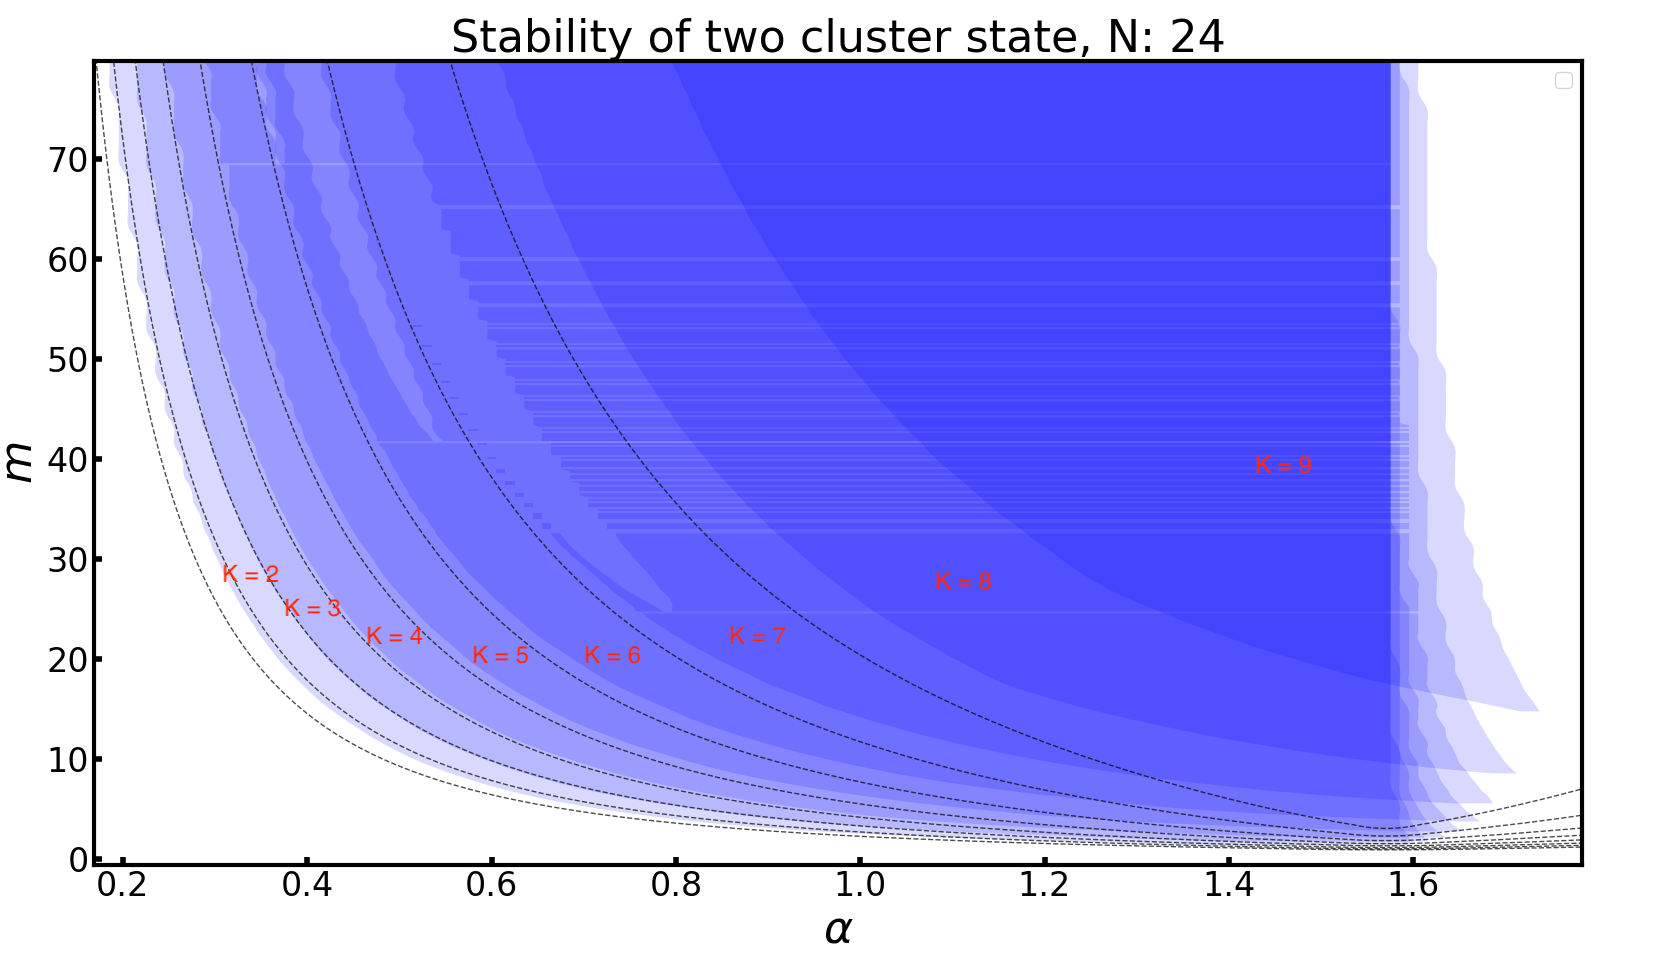
\includegraphics[width=1\columnwidth]{pictures/st-map.png}
		\end{center}
		\caption{\textbf{Карта устойчивости двух кластерных вращательных состояний с периодической расстройкой фаз в зависимости от параметра $\beta$.}
		Внутри синей зоны двух кластерный режим является устойчивым.
		$\beta = 0.494$}
	\end{figure}

\end{chapter}